%\documentclass[a4paper,twoside,11pt]{report} %openright
\documentclass[a4paper,oneside,11pt]{report} % will work also as a one-sided document


% Report type and number
%\newcommand{\documenttype}{BYG report}
\newcommand{\reportnumber}{BYG R-XXX} % For example "BYG R-432"
\newcommand{\thedate}{month, year} % For example "June, 2019"

% Report title
\newcommand{\reporttitle}{Report title}
\newcommand{\reportsubtitle}{Report subtitle}    % comment or leave blank if no sub-title

% report authors
\newcommand{\reportauthors}{Author1, Author2 \& Author3 }
\newcommand{\qcby}{Lars Larsen}                       % Specify who quality checked the report, comment or leave blank if not needed

% ISSN / ISBN information
\newcommand{\reportISSNelectronic}{0000-0000}         % ISSN for electronic version, comment if not needed/known
\newcommand{\reportISBNelectronic}{000-00-0000-000-0} % ISBN for electronic version, comment if not needed/known
%\newcommand{\reportISSNprinted}{0000-0000}            % ISSN for printed version, comment if not needed/known
%\newcommand{\reportISBNprinted}{000-00-0000-000-0}    % ISBN for printed version, comment if not needed/known

% Department information and address
\newcommand{\department}{DTU Civil Engineering}
\newcommand{\departmentdescriber}{Department of Civil Engineering}
\newcommand{\addressI}{Brovej, Building 118}
\newcommand{\addressII}{2800~Kgs. Lyngby}       % mbox used to prevent hyphenation
\newcommand{\departmentwebsite}{www.byg.dtu.dk}
\newcommand{\departmentphone}{+45 4525 1700}

% Cover image information
\newcommand{\coverimage}{./Pictures/DTU_stock_photo.jpg}
\newcommand{\coverimagedescription}{...write photo credits or description here...}

% Title image will be cropped to the predefined image box.
% Use settings below to control its size (zoom) and relative position in box
\newcommand{\coverimagewidth}{\paperwidth}    % use \paperwidth to scale image to width of the paper, or use a specific measure e.g. 30cm or 10cm to scale up or down 
\newcommand{\coverimagedx}{0cm}     % use 0cm to have image centered, positive value moves image left
\newcommand{\coverimagedy}{-2cm}    % use 0cm to have image centered, positive value moves image down


% Back page text description
\newcommand{\backpagetextdescription}{\blindtext}   % comment out, or replace \blindtext with own description to be shown on backpage


% -------------------------------------------------------------
% Some switches that will affect compilation of the document
% -------------------------------------------------------------
\newif\ifneosanspro     % define switch to control if NeoSansPro font is used for headings

% The DTU design team has proposed to use Neo Sans for headings - and Arial for the body text.
% The NeoSansPro font is not freely distributable and must be obtained from the DTU design team 
% see https://www.designguide.dtu.dk/standard-design-basics#standard-user-typography-banner
% 
% To use NeoSansPro please upload both NeoSansPro-Regular.otf and NeoSansPro-Medium.otf to the root directory
% of the project (same folder as main.tex), and set the switch below to true

%\neosansprotrue         % Use the NeoSansPro font (make sure it is available!)
\neosansprofalse        % Fall back to using Arial or other Sans Serif font



\newif\ifappendices     % define switch to control if appendices are included in the compilation or not
\appendicestrue         % include appendices
%\appendicesfalse        % don't include appendices    % Setup title, authors etc. in this file
%\usepackage{microtype}      % better looking text
%\usepackage[utf8]{inputenc}
\usepackage{fontspec}       % Package for custom fonts
\usepackage[]{geometry}     % Package for changing page margins (before fancyhdr) 
\usepackage{fancyhdr}       % Package to change header and footer
\usepackage{parskip}        % Package to tweak paragraph skipping (instead of indents a small skip is added after every paragraph)
\usepackage{titlesec}
\usepackage{tikz}           % Package for drawing
\usepackage{pgfplots}       % Package for creating graphs and charts
\usepackage{xcolor}         % Package for defining DTU colours to be used
\usepackage{amsmath}        % For aligning equations among other
\usepackage{siunitx}        % SI units
\usepackage{listings}       % Package for inserting code, (before cleveref)
\PassOptionsToPackage{hyphens}{url} % Ability to line break urls at hyphens
\usepackage{hyperref}       % Package for cross referencing (also loads url package)
\usepackage{cleveref}       % improved cross referencing
\usepackage{textcomp}       % \textdegree = °C and other useful symbols
\usepackage[english]{babel} % localisation 
\usepackage{caption}        % better captions
\usepackage{subcaption}     % for subfigures
\usepackage{csquotes}       % For biblatex with babel
\usepackage[backend=biber,style=authoryear,sorting=none]{biblatex} % Package for bibliography (citing)
\bibliography{bibliography.bib}
\usepackage{tabularx}       % for ability to adjust column spacing in tabular better
\usepackage{booktabs}       % for better tables
\usepackage{float}          % floating figures in correct places
\usepackage{calc}           % Adds ability for latex to calculate (3pt+2pt) 
% \usepackage[printwatermark=false]{xwatermark} % Package for wartermark. Toggle printwatermark true or false to include or remove the watermark
\usepackage{blindtext}

   % all usepackage statements go in this file
% Colours! 
\newcommand{\targetcolourmodel}{cmyk} % rgb for a digital version, cmyk for a printed version. Only use lowercase
\selectcolormodel{\targetcolourmodel}

% Define colours from https://www.designguide.dtu.dk/
\definecolor{dtured}    {rgb/cmyk}{0.6,0,0 / 0,0.91,0.72,0.23}
\definecolor{blue}      {rgb/cmyk}{0.1843,0.2431,0.9176 / 0.88,0.76,0,0}
\definecolor{brightgreen}{rgb/cmyk}{0.1216,0.8157,0.5098 / 0.69,0,0.66,0}
\definecolor{navyblue}  {rgb/cmyk}{0.0118,0.0588,0.3098 / 1,0.9,0,0.6}
\definecolor{yellow}    {rgb/cmyk}{0.9647,0.8157,0.3019 / 0.05,0.17,0.82,0}
\definecolor{orange}    {rgb/cmyk}{0.9882,0.4627,0.2039 / 0,0.65,0.86,0}
\definecolor{pink}      {rgb/cmyk}{0.9686,0.7333,0.6941 / 0,0.35,0.26,0}
\definecolor{grey}      {rgb/cmyk}{0.8549,0.8549,0.8549 / 0,0,0,0.2}
\definecolor{red}       {rgb/cmyk}{0.9098,0.2471,0.2824 / 0,0.86,0.65,0}
\definecolor{green}     {rgb/cmyk}{0,0.5333,0.2078 / 0.89,0.05,1,0.17}
\definecolor{purple}    {rgb/cmyk}{0.4745,0.1373,0.5569 / 0.67,0.96,0,0}

\newcommand{\dtulogocolour}{white} % Colour of the DTU logo: white, black or dtured
\newcommand{\frontpagetextcolour}{white} % front page text colour: white or black
\colorlet{frontbackcolor}{blue} % Set the background colour of the front- and back page. Choose the colour so it matches the main colour of front page picture

% DTU colours for diagrams
% You might want to make the front/back page background colour the first colour in the plot cycle list.
\pgfplotscreateplotcyclelist{DTU}{%
dtured,         fill=dtured,        \\%
blue,           fill=blue,          \\%
brightgreen,    fill=brightgreen    \\%
navyblue,       fill=navyblue       \\%
yellow,         fill=yellow         \\%
orange,         fill=orange         \\%
grey,           fill=grey           \\%
red,            fill=red            \\%
green,          fill=green          \\%
purple,         fill=purple         \\%
}


% Font
% There is no corporate serif font in the DTU design guide. The DTU design team has proposed to use Neo Sans for headings - and Arial for the body text.
% To change heading font to NeoSans Pro please upload both NeoSansPro-Regular.otf and NeoSansPro-Medium.otf to the root directory.
\setmainfont{Arial}
\renewcommand\thepart{Part \Roman{part}}
\IfFontExistsTF{NeoSansPro-Medium.otf}
{ %If True set headings to NeoSans Pro
\newfontface\NeoSansProReg{NeoSansPro-Regular.otf}
\newfontface\NeoSansProMed{NeoSansPro-Medium.otf}
\titleformat{\part}[display]{\NeoSansProMed \huge \centering}{\NeoSansProMed \Huge \thepart}{1em}{\thispagestyle{empty}}{}
\titleformat{\chapter}{\NeoSansProMed\huge}{\thechapter}{1em}{\raggedright}
\titleformat{\section}{\NeoSansProMed\Large}{\thesection}{1em}{\raggedright}
\titleformat{\subsection}{\NeoSansProMed\large}{\thesubsection}{1em}{\raggedright}
\titleformat{\subsubsection}{\NeoSansProMed\normalsize}{\thesubsubsection}{1em}{\raggedright}
\newcommand\TitleFont[1]{{\NeoSansProMed #1}}
\newcommand\titlefont[1]{{\NeoSansProReg #1}}
}
{ % If false
\titleformat{\part}[display]{\bfseries\huge \centering}{\bfseries\Huge \thepart}{1em}{\thispagestyle{empty}}{}
\titleformat{\chapter}{\bfseries\huge}{\thechapter}{1em}{\raggedright}
\titleformat{\section}{\bfseries\Large}{\thesection}{1em}{\raggedright}
\titleformat{\subsection}{\bfseries\large}{\thesubsection}{1em}{\raggedright}
\titleformat{\subsubsection}{\bfseries\normalsize}{\thesubsubsection}{1em}{\raggedright}
\newcommand\TitleFont[1]{{\bfseries #1}}
\newcommand\titlefont[1]{{#1}}
}
\urlstyle{sf}
%\def\UrlFont{\NeoSansProReg}


% If you wish to use the pdflatex compiler, sans-serif Helvetica can be used as a replacement for Arial. In this way you will be able to use the microtype package. Remember to add \usepackage[utf8]{inputenc} and disable the fontspec package. 
%\newcommand\TitleFont[1]{{\bfseries #1}}
%\newcommand\titlefont[1]{{#1}}
%\fontfamily{qhv}\selectfont
%\renewcommand{\familydefault}{\sfdefault}


% Watermark for confidential or draft (or anything else)
%\sffamily % set the correct font for the watermark
\newsavebox\mybox
\savebox\mybox{\tikz[color=grey,opacity=0.5]\node{Template};}

\newwatermark*[
  oddpages,
  angle=60,
  scale=12,
  %fontfamily=qhv,
  xpos=-40,
  ypos=30,
]{\usebox\mybox}

\newwatermark*[
  evenpages,
  angle=60,
  scale=12,
  %fontfamily=qhv,
  xpos=-50,
  ypos=30,
]{\usebox\mybox}


% Table of contents (TOC) and numbering of headings
\setcounter{tocdepth}{1}    % Depth of table of content: sub sections will not be included in table of contents
\setcounter{secnumdepth}{2} % Depth of section numbering: sub sub sections are not numbered

\makeatletter % Reset chapter numbering for each part
\@addtoreset{chapter}{part}
\makeatother  

% Spacing of titles and captions
\titlespacing\chapter{0pt}{0pt plus 4pt minus 2pt}{4pt plus 2pt minus 2pt}
\titlespacing\section{0pt}{12pt plus 3pt minus 3pt}{2pt plus 1pt minus 1pt}
\titlespacing\subsection{0pt}{8pt plus 2pt minus 2pt}{0pt plus 1pt minus 1pt}
\titlespacing\subsubsection{0pt}{4pt plus 1pt minus 1pt}{-2pt plus 1pt minus 1pt}
\captionsetup{belowskip=\parskip,aboveskip=4pt plus 1pt minus 1pt}

% Setup header and footer
\fancypagestyle{main}{% All normal pages
    \fancyhead{}
    \fancyfoot{}
    \renewcommand{\headrulewidth}{0pt}
    \fancyfoot[LE,RO]{\footnotesize \thepage}
    \fancyfoot[RE,LO]{\footnotesize \thesistitle} % - \rightmark
    \fancyhfoffset[E,O]{0pt}
}
\fancypagestyle{plain}{% Chapter pages
    \fancyhead{}
    \fancyfoot{}
    \renewcommand{\headrulewidth}{0pt}
    \fancyfoot[LE,RO]{\footnotesize \thepage}
    \fancyfoot[RE,LO]{\footnotesize \thesistitle} % - \leftmark
    \fancyhfoffset[E,O]{0pt}
}


% Setup for diagrams and graphs (tikz pictures) 
\usetikzlibrary{spy}    % For magnifying anything within a tikzpicture, see the line graph
\usepgfplotslibrary{statistics} % Package for the boxplot
\pgfplotsset{ % Setup for diagrams
compat=newest,
major x grid style={line width=0.5pt,draw=grey},
major y grid style={line width=0.5pt,draw=grey},
legend style={at={(0.5,-0.1)}, anchor=north,fill=none,draw=none,legend columns=-1,/tikz/every even column/.append style={column sep=10pt}},
axis line style={draw=none},
tick style={draw=none},
every axis/.append style={ultra thick},
tick label style={/pgf/number format/assume math mode}, % To apply main font to tick labels (numbers on the axis)
}
\tikzset{every mark/.append style={scale=1.5}}


% Hypersetup
\hypersetup{
    pdfauthor={\thesisauthor},
    pdftitle={\thesistitle},
    pdfsubject={\thesissubtitle},
    pdfdisplaydoctitle,
    bookmarksnumbered=true,
    bookmarksopen,
    breaklinks,
    linktoc=all,
    plainpages=false,
    unicode=true,
    colorlinks=false,
    hidelinks,                        % Do not show boxes or coloured links.
}


% Listings setup
\lstset{
    basicstyle=\footnotesize\ttfamily,% the size of the fonts that are used for the code
    commentstyle=\color{green},       % comment style
    keywordstyle=\bfseries\ttfamily\color{blue}, % keyword style
    numberstyle=\sffamily\tiny\color{grey}, % the style that is used for the line-numbers
    stringstyle=\color{purple},       % string literal style
    rulecolor=\color{grey},           % if not set, the frame-color may be changed on line-breaks within not-black text (e.g. comments (green here))
    breakatwhitespace=false,          % sets if automatic breaks should only happen at whitespace
    breaklines=true,                  % sets automatic line breaking
    captionpos=b,                     % sets the caption-position to bottom
    deletekeywords={},                % if you want to delete keywords from the given language
    escapeinside={\%*}{*)},           % if you want to add LaTeX within your code
    frame=single,                     % adds a frame around the code
    xleftmargin=4pt, 
    morekeywords={*,...},             % if you want to add more keywords to the set
    numbers=left,                     % where to put the line-numbers; possible values are (none, left, right)
    numbersep=10pt,                   % how far the line-numbers are from the code
    showspaces=false,                 % show spaces everywhere adding particular underscores; it overrides 'showstringspaces'
    showstringspaces=false,           % underline spaces within strings only
    showtabs=false,                   % show tabs within strings adding particular underscores
    stepnumber=1,                     % the step between two line-numbers. If it's 1, each line will be numbered
    tabsize=2,                        % sets default tabsize to 2 spaces
    title=\lstname,                   % show the filename of files included with \lstinputlisting; also try caption instead of title
}

% Signature field
\newlength{\myl}
\newcommand{\namesigdatehrule}[1]{\par\tikz \draw [black, densely dotted, very thick] (0.04,0) -- (#1,0);\par}
\newcommand{\namesigdate}[2][]{%
\settowidth{\myl}{#2}
\setlength{\myl}{\myl+10pt}
\begin{minipage}{\myl}%
\begin{center}
    #2  % Insert name from the command eg. \namesigdate{\authorname}
    \vspace{1.5cm} % Spacing between name and signature line 
    \namesigdatehrule{\myl}\smallskip % Signature line and a small skip
    \small \textit{Signature} % Text under the signature line "Signature"
    \vspace{1.0cm} % Spacing between "Signature" and the date line
    \namesigdatehrule{\myl}\smallskip % Date line and a small skip
    \small \textit{Date} % Text under date line "Date" 
\end{center}
\end{minipage}
}

% For the back page: cleartoleftpage
\newcommand*\cleartoleftpage{%
  \clearpage
  \ifodd\value{page}\hbox{}\newpage\fi
}
   % additional definitions here, changes should not be necessary 

\begin{document}

\pagenumbering{roman}
\title{\thesistitle} 
\author{\thesisauthor} 
\date{\thedate} 

\begin{titlepage}

\newgeometry{left=11mm,right=11mm,top=50mm,bottom=0pt}
\pagecolor{frontbackcolor}
\color{\frontpagetextcolour}

{ % Thesis title (to change see Setup/Settings.tex) 
\Huge
\begin{tabular}{p{.9\textwidth}}
\TitleFont{\thesistitle}   \\ 
\TitleFont{\thesissubtitle} \bigskip \\ 
\titlefont{\documenttype}
\end{tabular}
}

% DTU department (to change see Setup/Settings.tex) 
\begin{tikzpicture}[remember picture,overlay]
\node[anchor=north east, 
      xshift=-10mm, 
      yshift=-12mm] 
      at (current page.north east) 
      {
        \color{\frontpagetextcolour}
        \begin{tabular}{r} 
        \textbf{\department} \\ 
        \departmentdescriber
        \end{tabular}
      }; 
\end{tikzpicture}

% DTU logo
\begin{tikzpicture}[remember picture,overlay]
\node[anchor=north west, 
      xshift=8.9mm, 
      yshift=-8.3mm] 
     at (current page.north west) 
     {\includegraphics[width=14.75mm,keepaspectratio]{Pictures/Logos/\dtulogocolour_\targetcolourmodel.pdf}}; 
\end{tikzpicture}

% Cover photo
\begin{tikzpicture}[remember picture,overlay]
\node[anchor=south, % anchor is bottom of picture
      xshift=0pt, 
      yshift=-2.9mm] % shifting picture to actually be at the bottom of the page
     at (current page.south) % placement at bottom of the page
     {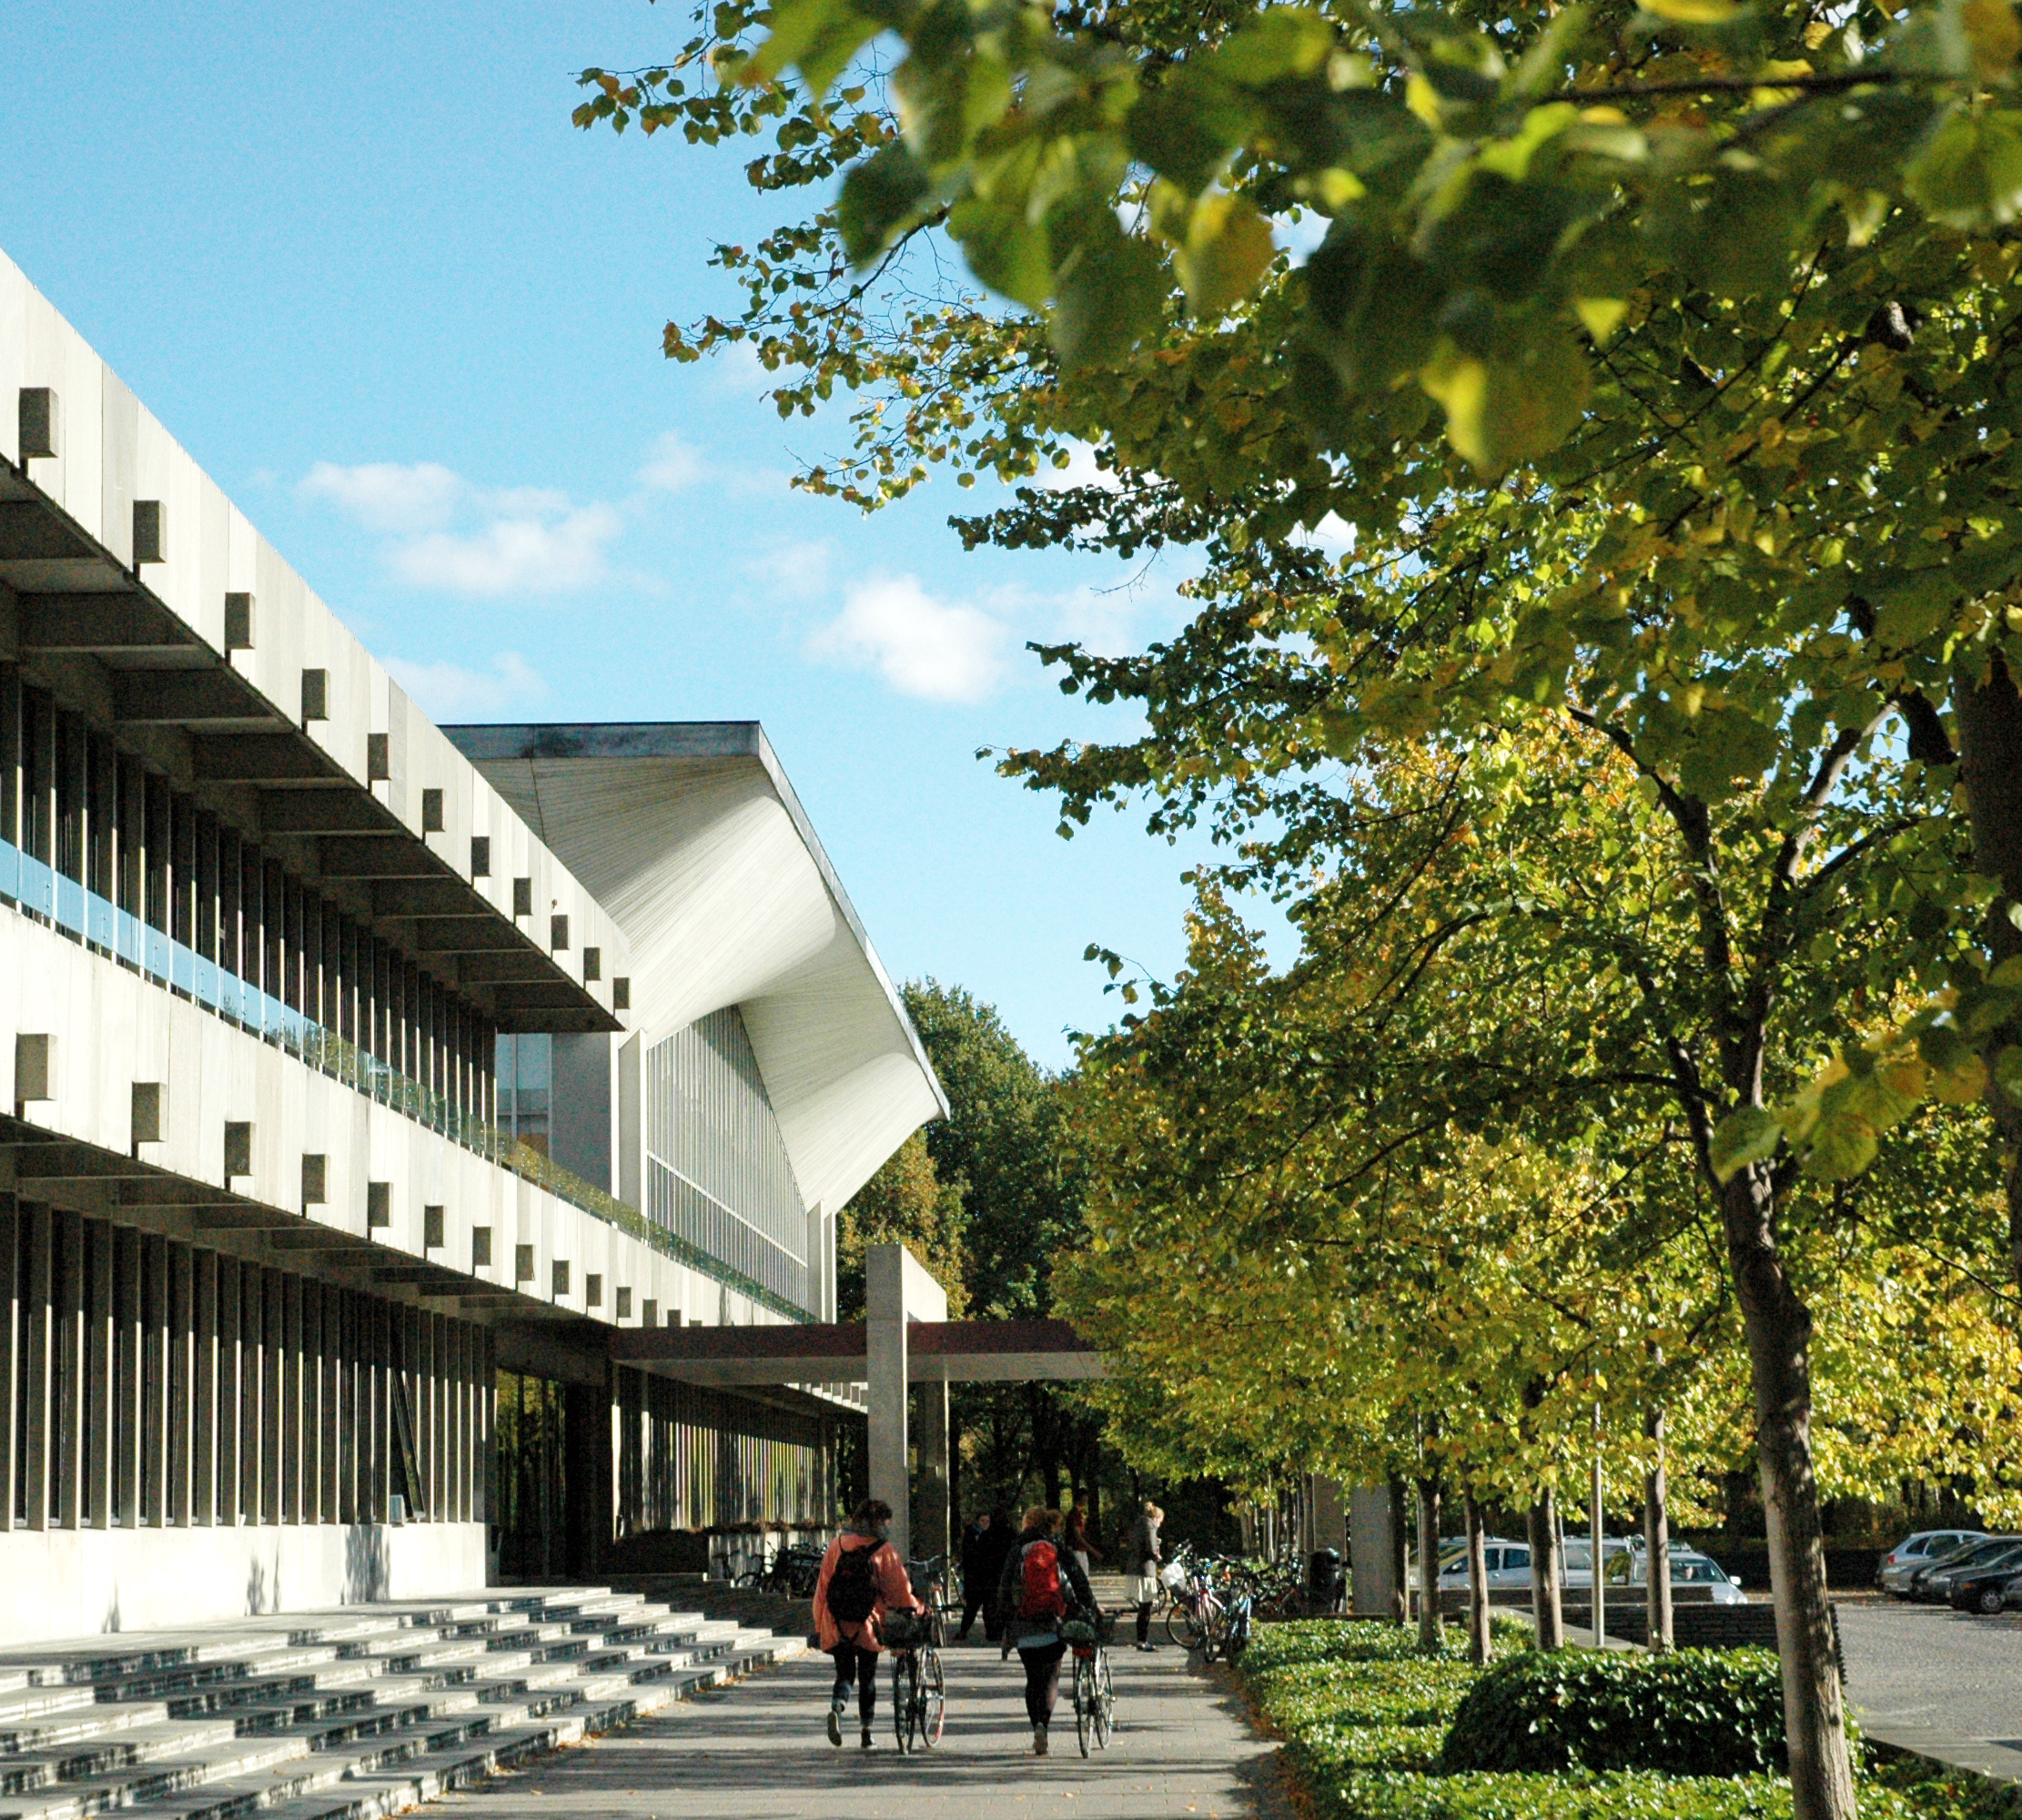
\includegraphics[height=18.9cm,keepaspectratio]{Pictures/DTU_stock_photo.jpg}};
\end{tikzpicture}




\end{titlepage}

\pagecolor{white}
\newgeometry{top=2.81cm, bottom=2.75cm, outer=2.5cm, inner=3.5cm}
\pagestyle{empty}
\cleardoublepage 
\thispagestyle{empty}
\setcounter{page}{1}
\vspace*{\fill}

\textbf{\reporttitle} \newline
\ifdefined\reportsubtitle
	\reportsubtitle
\fi

\smallskip

\ifdefined\documenttype
	\documenttype \newline
\fi
\ifdefined\reportnumber
	\reportnumber \newline
\fi
\thedate

\smallskip

By \newline
\reportauthors

\bigskip

\begin{tabularx}{\textwidth}{@{}l>{\raggedright\arraybackslash}X@{}}
    Copyright: & Reproduction of this publication in whole or in part must include the customary bibliographic citation, including author attribution, report title, etc. \\
    &\\
    \ifdefined \coverimage
    \ifdefined \coverimagedescription
    Cover image: & \coverimagedescription \\
    & \\
    \fi
    \fi
    Published by: & DTU, \mbox{\departmentdescriber}, \mbox{\addressI}, \mbox{\addressII},~Denmark  \\
    & \url{\departmentwebsite} \\
    & \\
    \ifdefined \reportISSNelectronic
	    ISSN: & \reportISSNelectronic ~(electronic version) \\
 	\fi
 	\ifdefined \reportISBNelectronic
    ISBN: & \reportISBNelectronic ~(electronic version) \\
    \fi
    & \\
    \ifdefined \reportISSNprinted
	    ISSN: & \reportISSNprinted ~(printed version) \\
 	\fi
 	\ifdefined \reportISBNprinted
	    ISBN: & \reportISBNprinted ~(printed version) \\
 	\fi
\end{tabularx}



\clearpage 
\pagestyle{main}
%\section*{Approval}
\addcontentsline{toc}{section}{Preface}
This thesis has been prepared over six months at the Section for Indoor Climate, Department of Civil Engineering, at the Technical University of Denmark, DTU, in partial fulfilment for the degree Master of Science in Engineering, MSc Eng. 

It is assumed that the reader has a basic knowledge in the areas of statistics. 

\vfill

\begin{center}
\namesigdate{\thesisauthor~-~\studentnumber}
\end{center}

\vfill


%\clearpage 
\section*{Abstract}
\addcontentsline{toc}{section}{Abstract}

\blindtext






\clearpage 
\section*{Acknowledgements}
\addcontentsline{toc}{section}{Acknowledgements}

\blindtext

\cleardoublepage 
\tableofcontents
\cleardoublepage 

%%%%%%%%%%%%%%%%%%%%%%%%%%%%%%%%%%%%%%%%%%%%%%%%%%%%%%%
\pagenumbering{arabic}
\chapter{Introduction}
This template complies with the DTU Design Guide \url{https://www.designguide.dtu.dk/}. DTU holds all rights to the design programme including all copyrights. It is intended for two-sided printing. The \textbackslash \texttt{cleardoublepage} command can be used to ensure that new sections and the table of contents begins on a right hand page. The back page always ends as an odd page. 

All document settings have been gathered in Setup/Settings.tex. These are global settings meaning the settings will affect the whole document. Defining the title for example will change the title on the front page, the copyright page and the footer. A watermark can be enabled or disabled in Setup/Premeable.tex. You can edit the watermark to display draft, review, approved, confidential or anything else. By default the watermark is printed on top of the contents of the document and has a transparent grey colour. 

\section{This is a section}
Every chapter is numbered and the sections inherit the chapter number followed by a dot and a section number. Figures, equations, tables, ect. also inherit the chapter numbering. 

\subsection{This is a sub section}
Sub sections are also numbered. In general try not to use a deep hierarchy of sub sections (\texttt{\textbackslash paragraph\{\}} and the like). The document will become segmented which will make the document appear less coherent. 

\subsubsection{This is a sub sub section}
And those are not numbered. It is possible to adjust how deep hierarchy of numbering sections goes in Setup/Settings.tex. 

The front and back cover have been made to replicate the examples in the design guide \url{https://www.designguide.dtu.dk/#stnd-printmedia}. The name of department heading is omitted  because it is located in the top right corner (no need to write it twice). Take a look at \url{https://www.inside.dtu.dk/en/medarbejder/om-dtu-campus-og-bygninger/kommunikation-og-design/skabeloner/rapporter} if you want to make your cover separately. 

Citing is done with the \texttt{biblatex} package \cite{biblatex}. Cross referencing (figures, tables, ect.) is taken care by the \texttt{cleveref} package. Just insert the name of the label in \textbackslash \texttt{cref\{\}} and it will automatically format the cross reference. For example writing the \texttt{cleveref} command \textbackslash \texttt{cref\{fig:groupedcolumn\}} will output ``\cref{fig:groupedcolumn}''. Using \textbackslash \texttt{Cref\{\}} will capitalise the first letter and \textbackslash \texttt{crefrange\{\}\{\}} will make a reference range. An example: \Cref{fig:stackedbar} is an example of a stacked bar chart and \crefrange{fig:stackedcolumn}{fig:groupedcolumn} are three consecutive figures.

\section{Font and symbols test}
Symbols can be written directly in the document meaning there is no need for special commands to write special characters. I love to write special characters like æøå inside my \TeX{} document. Also á, à, ü, û, ë, ê, î, ï could be nice. So what about the ``¿'' character. What about ° é ® † ¥ ü | œ ‘ @ ö ä ¬ ‹ « © ƒ ß ª … ç ñ µ ‚ · ¡ “ £ ™ [ ] '. Some dashes - – —, and the latex form - -- --- 

This is a font test \newline 
Arial Regular \newline 
\textit{Arial Italic} \newline 
\textbf{Arial Bold} \newline 
\textbf{\textit{Arial Bold Italic}}

\cleardoublepage 
\chapter{Colours} \label{sec:colours}
The design guide define 3 primary colours (dtured, white and black) and 10 secondary colours \url{https://www.designguide.dtu.dk/#stnd-colours}. Below are codes for the various colour modes. RGB is used for web and Office Programmes. CMYK is used for print. HTML is used for HTML-coding. If you know anything about colour codes you might notice that the RGB codes are ranging from 0-1 instead of the usual 0-255. 

\begin{testcolors}[rgb,cmyk,HTML]
\testcolor{dtured}
\testcolor{white}
\testcolor{black}
\testcolor{blue}
\testcolor{brightgreen}
\testcolor{navyblue}
\testcolor{yellow}
\testcolor{orange}
\testcolor{pink}
\testcolor{red}
\testcolor{green}
\testcolor{purple}
\end{testcolors}

The default colour mode for this template is cmyk. The current colour model is \targetcolourmodel~which is also illustrated by the underlined numbers in the colour test table above.  If you which to change the colour model to rgb go to Setup/Settings.tex and change \texttt{targetcolourmodel} to rgb. In Setup/Settings.tex it is also possible to change the background colour of the front and back page. The colours are primarily used for diagrams (the plotcyclelist DTU) and the front and back page.

Lighter colours can be achieved as written in the \LaTeX{} code below. For example to get a tint of 50\% you would write colourname!50.  \newline
{\raggedright
\textcolor{dtured}{Normal dtured} \qquad
\textcolor{dtured!80}{80\% dtured} \qquad 
\textcolor{dtured!70}{70\% dtured} \qquad
\textcolor{dtured!60}{60\% dtured} \qquad
\textcolor{dtured!50}{50\% dtured} 
}
\newline
For more information about colours in \LaTeX{} read the \texttt{xcolor} manual.


\cleardoublepage 
\chapter{Examples of figures, tables, equations and listings}
In the following a bunch of examples of figures and tables have been made. There are advantages to using \texttt{tikZ} diagrams over excel diagrams. 1) the font and font size perfectly matches the document 2) the styling and colours are pre-defined to follow the design guide 3) the plots uses vector graphics which reduces the file size, reduces the compile time and looks sharp when zooming in. The possibilities are endless, look at the \texttt{pgfplots} gallery for inspiration: \url{http://pgfplots.sourceforge.net/gallery.html}. 
However there are still cases where I would recommend to insert a plot as a picture. For example if the plot contains a lot of data: a line graph with 1000 points takes a long time to compile. 

Some tips if you want good looking diagrams or graphs which will be inserted as pictures (e.g. in a figure environment with \textbackslash includegraphics): The main font is Arial. Use DTU colours as described in \cref{sec:colours}. Use high quality pictures. Try to scale the diagram (picture) so the text size of the axis legends match the text size in this document.

Remember to change the label of your figures so there are no duplicate labels. A label should be placed below a caption or after a heading (fx after a \textbackslash chapter). 





\section{Graphs and charts}

\pgfplotstableread{
x  {Name 1} {Name 2}    {Name 3}    {Name 4}
1  0.847    0.786       0.367       0.742
2  1.73     0.838       1.27        1.05
3  1.50     0.952       0           0
4  0.506    1.05        0.751       0.698
5  0.672    0.777       0           0
6  0.349    1.62        1.16        0.655
7  0.498    0.480       0.375       0.306
8  0.454    0.925       0.498       0.375
9  0.698    0.716       0.733       0.541
10 0.829    1.12        0.803       0.725
}\stackedColumnData

\begin{figure}[htb]
\centering
\begin{tikzpicture} 
\begin{axis}[ 
    width=15cm, % You could use \linewidth instead 
    height=6.6cm,
    ybar stacked, 
    xtick = data,
    xticklabels={1,2,3,4,5,6,Var 1,Var 2,Var 3,Var 4},
    ylabel={Some text with a unit $\phi$ }, 
    ymajorgrids=true,
    legend style={at={(0.5,-0.1)}, anchor=north}, 
    cycle list name=DTU,
    every axis plot/.append style={fill,draw=none},
    ] 
\addplot table[x=x,y={Name 1}]{\stackedColumnData}; 
\addplot table[x=x,y={Name 2}]{\stackedColumnData};
\addplot table[x=x,y={Name 3}]{\stackedColumnData};
\addplot table[x=x,y={Name 4}]{\stackedColumnData};
\legend{Heating,Ventilation,Lighting,Solar shading} 
\end{axis} 
\end{tikzpicture}
\caption{Stacked column chart}
\label{fig:stackedcolumn}
\end{figure}



\pgfplotstableread{
y {Name 1} {Name 2} {Name 3} {Name 4} 
1 50        20      15       15
2 10        40      25       25
3 40        30      20       10
4 30        10      20       40
5 30        20      10       40
6 20        10      40       30
7 10        10      50       30
}\stackedBarData

\begin{figure}[H]%
\centering
\begin{tikzpicture}
\begin{axis}[
    width=15cm-10pt, % pgfplots widths are only approximate. You might have to fine tune the width of your figures to deal with overfull hbox warnings. 
    height = 6.6cm,
    xbar stacked,
    xlabel=Write something here,
    ytick=data,
    yticklabels = {Text 1, Text 2, Text 3, Text 4, Text 5, Text 6, Text 7},
    xmin = 0,
    enlarge x limits=false,
    xmajorgrids=true,
    legend style={at={(0.5,-0.22)}},
    cycle list name=DTU,
    every axis plot/.append style={fill,draw=none},
    ]
\addplot table[x={Name 1},y=y]{\stackedBarData};
\addplot table[x={Name 2},y=y]{\stackedBarData};
\addplot table[x={Name 3},y=y]{\stackedBarData};
\addplot table[x={Name 4},y=y]{\stackedBarData};
\legend{Legend 1, Legend 2, Legend 3, Legend 4} 
\end{axis}  
\end{tikzpicture}
\caption{Stacked bar chart}
\label{fig:stackedbar}
\end{figure}



\pgfplotstableread{
x    {Far}  {Near}  {Here}
1930 50     38      15
1940 33     42      12
1950 40     43      13
1960 50     45      25
1970 70     65      35
}\groupedColumnData

\begin{figure}[H]
\centering
\begin{tikzpicture} 
\begin{axis}[ 
    width=15cm,
    height=6.6cm,
    ybar,
    xtick=data,
    x tick label style={ /pgf/number format/1000 sep=}, 
    ylabel=Population,  
    ymin=0,
    ymajorgrids=true,
    legend style={at={(0.5,-0.15)},anchor=north,legend columns=-1},
    cycle list name=DTU, 
    ] 
\addplot table[x=x,y={Far}]{\groupedColumnData}; 
\addplot table[x=x,y={Near}]{\groupedColumnData};
\addplot table[x=x,y={Here}]{\groupedColumnData}; 
\addplot[red,sharp plot,update limits=false] coordinates {(1910,43) (1990,43)} node[above] at (axis cs:1950,43) {Houses}; 
\legend{Far,Near,Here,Annot} 
\end{axis} 
\end{tikzpicture}
\caption{Grouped column chart}
\label{fig:groupedcolumn}
\end{figure}



\pgfplotstableread{
x {Name 1} {Name 2} {Name 3} {Name 4} 
1 0         10       58       10
2 30        20       48       40
3 10        60       45       10.5
4 50        18       55       60
5 40        30       8        20
}\lineGraphData

\begin{figure}[H]
\centering
\begin{tikzpicture}[spy using outlines = {circle, size=2cm, magnification=5, connect spies}]
\begin{axis}[
    width=15cm,
    height=6.6cm,
    ylabel = {Unit},
    ymin = 0,
    enlarge x limits = false,
    ymajorgrids = true,
    legend style = {at={(0.5,-0.1)}, anchor=north},
    cycle list name=DTU,
    every axis plot/.append style={fill opacity=0},
    ] 
\addplot table[x=x,y={Name 1}]{\lineGraphData}; 
\addplot table[x=x,y={Name 2}]{\lineGraphData};
\addplot table[x=x,y={Name 3}]{\lineGraphData}; 
\addplot table[x=x,y={Name 4}]{\lineGraphData}; 
\legend{Legend 1, Legend 2, Legend 3, Legend 4} 
\end{axis} 
\end{tikzpicture}
\caption{Line graph}
\label{fig:linegraph}
\end{figure}



\pgfplotstableread{
x {Name 1} {Name 2} {Name 3} {Name 4} 
1 0         10       58       10
2 30        20       48       40
3 10        60       45       10.5
4 50        18       55       60
5 40        30       8        20
}\lineGraphMagnifyData

\begin{figure}[H]
\centering
\begin{tikzpicture}[spy using outlines = {circle, size=2cm, magnification=5, connect spies}]
\begin{axis}[
    width=15cm,
    height=6.6cm,
    ylabel = {Unit},
    ymin = 0,
    enlarge x limits = false,
    ymajorgrids = true,
    legend style = {at={(0.5,-0.1)}, anchor=north},
    cycle list name=DTU,
    every axis plot/.append style={fill opacity=0},
    ] 
\addplot table[x=x,y={Name 1}]{\lineGraphMagnifyData}; 
\addplot table[x=x,y={Name 2}]{\lineGraphMagnifyData};
\addplot table[x=x,y={Name 3}]{\lineGraphMagnifyData}; 
\addplot table[x=x,y={Name 4}]{\lineGraphMagnifyData}; 

\coordinate (spypoint) at (axis cs:3,10.5); % Delete this line to remove magnifying glass
\coordinate (magnifyglass) at (axis cs:3.6,12); % Delete this line to remove magnifying glass
\legend{Legend 1, Legend 2, Legend 3, Legend 4} 
\end{axis} 

\spy [black, size=2cm] on (spypoint) in node[fill=white] at (magnifyglass); % Delete this line to remove magnifying glass
\end{tikzpicture}
\caption{Line graph with magnifying glass}
\label{fig:linegraphmagnify}
\end{figure}



\pgfplotstableread{
x {Name 1} {Name 2} {Name 3} {Name 4} 
1 30        10       2        10
2 20        20       5        5
3 25        20       5        8
4 15        20       5        5
5 30        10       8        2
}\areaGraphData

\begin{figure}[H]
\centering
\begin{tikzpicture} 
\begin{axis}[
    width=15cm,
    height=6.6cm,
    stack plots=y, 
    area style,
    ylabel = {Unit},
    ymin = 0,
    enlarge x limits=false,
    ymajorgrids=true,
    legend style={at={(0.5,-0.1)}, anchor=north}, 
    cycle list name=DTU,
    ] 
\addplot table[x=x,y={Name 1}]{\areaGraphData}\closedcycle; 
\addplot table[x=x,y={Name 2}]{\areaGraphData}\closedcycle;
\addplot table[x=x,y={Name 3}]{\areaGraphData}\closedcycle; 
\addplot table[x=x,y={Name 4}]{\areaGraphData}\closedcycle; 
\legend{Legend 1, Legend 2, Legend 3, Legend 4} 
\end{axis} 
\end{tikzpicture}
\caption{Area graph}
\label{fig:areagraph}
\end{figure}



\pgfplotstableread{
x {Name 1} {Name 2} {Name 3} {Name 4} 
1   11	15	38	41
2   33	22	25	31
3   22	25	11	21
4   44	14	17	51
5   13	42	25	33
6   14	52	36	34
}\scatterData

\begin{figure}[H]
\centering
\begin{tikzpicture}
\begin{axis}[
    %enlarge x limits=true,
    ylabel = {Unit},
    ymin = 0,
    ymajorgrids=true,
    cycle list name=DTU,
]
\addplot+[only marks,mark=*]        table[x=x,y={Name 1}]{\scatterData};
\addplot+[only marks,mark=square*]  table[x=x,y={Name 2}]{\scatterData};
\addplot+[only marks,mark=triangle*]table[x=x,y={Name 3}]{\scatterData};
\addplot+[only marks,mark=+]        table[x=x,y={Name 4}]{\scatterData};
\legend{Legend 1, Legend 2, Legend 3, Legend 4} 
\end{axis}
\end{tikzpicture}
\caption{Scatter plot}
\label{fig:scatter}
\end{figure}


\begin{figure}[H]
\centering
\begin{tikzpicture}
\begin{axis}[
    boxplot/draw direction=y,
    xtick={1,2,3},
    xticklabels={Group A, Group B, Group C},
    x axis line style={opacity=0},
    enlarge y limits,
    ymajorgrids,
    cycle list name=DTU,
    every axis plot/.append style={semithick},
]
\addplot+[draw=black,
boxplot prepared={
lower whisker=42, lower quartile=45,
median=47,
upper quartile=47.5, upper whisker=48,
},
] coordinates {(0,40) (0,34) (0,56)};
\addplot+[draw=black,
boxplot prepared={
lower whisker=36, lower quartile=39,
median=40,
upper quartile=41, upper whisker=43,
},
] coordinates {};
\addplot+[draw=black,
boxplot prepared={
lower whisker=41, lower quartile=44,
median=45,
upper quartile=46, upper whisker=47,
},
] coordinates {(0,35) (0,55)};
\end{axis}
\end{tikzpicture}
\caption{Boxplot}
\label{fig:boxplot}
\end{figure}






\section{Tables and figures}

\begin{table}[H]
\centering
\caption{This is a \texttt{booktabs} table. Go to \url{http://www.tablesgenerator.com/} and use the booktabs table style}
\label{tab:tableExample}
\begin{tabular}{@{}llS@{}}
\toprule
\multicolumn{2}{c}{Item} &            \\ \cmidrule(r){1-2}
Animal     & Description & Price (\$) \\ \midrule
Gnat       & per gram    & 13.65      \\
           & each        & 0.01       \\
Gnu        & stuffed     & 92.50      \\
Emu        & stuffed     & 33.33      \\
Armadillo  & frozen      & 8.99       \\ \bottomrule
\end{tabular}
\end{table}
\texttt{Booktabs} tables don't use any vertical lines. Only horizontal lines are used. \Cref{tab:tableExample} begins with a \textbackslash \texttt{toprule}, ends with a \textbackslash \texttt{bottomrule} with \textbackslash \texttt{midrule} in between. The table has 3 columns formatted as \texttt{@\{\}llS@\{\}}. \texttt{@\{\}} is cropping the horizontal lines of the table to fit the content (removes column spacing at the left and right edges). \texttt{l} aligns the column to the left and \texttt{S} aligns the column according to the decimal point (\texttt{siunitx} package). You can of course also use \texttt{r} to align right or \texttt{c} to center the contents of the column. 

\begin{table}[H]
\centering
\caption{Wrongly formatted table}
\label{tab:tableExampleWrong}
\begin{tabular}{llll}
\toprule
                    & Voltage & Current   & Power   \\
                    & V       & A         & W       \\ \midrule
Transformer input   & 234.4   & 0.50      & 117.4   \\ \midrule
Transformer output  & 25.86   & 2.72      & 70.3    \\ \midrule
Efficiency          &         &           & 60\%    \\ \bottomrule
\end{tabular}
\end{table}

\begin{table}[H]
\centering
\caption{Correctly formatted table}
\label{tab:tableExampleCorrect}
\begin{tabular}{@{}lSSS@{}}
\toprule
                    & {Voltage} & {Current} & {Power}       \\
                    & V         & A         & W             \\ \midrule
Transformer input   & 234.4     & 0.50      & 117.4         \\ 
Transformer output  & 25.86     & 2.72      & 70.3          \\ \midrule
Efficiency          &           &           & \SI{60}{\percent} \\ \bottomrule
\end{tabular}
\end{table}

\Cref{tab:tableExampleWrong} and \cref{tab:tableExampleCorrect} have the same comtents but there are some subtle differences in formatting which makes \cref{tab:tableExampleCorrect} the superior table of the two. The most obvious change is removing the midrule between the transformer input and output rows. The efficency row is the odd man out and a midrule has been used to emphasise the difference between the transformer rows and the efficiency row. The delimiters in the voltage, current and power columns are aligned. The horizontal lines (rules) fits to the content and instead of protruding. The spacing between 60 and the percentage sign is correctly adjusted. 

\begin{figure}[H]
\centering

\includegraphics[width=0.3\textwidth]{Pictures/Logos/dtured_cmyk.pdf}
\caption{Just a normal figure}
\label{fig:figure}
\end{figure}



\begin{figure}[H]
\centering
\begin{subfigure}{.5\textwidth}
  \centering
  
\includegraphics[width=.4\linewidth]{Pictures/Logos/dtured_cmyk.pdf}
  \caption{A subfigure}
  \label{fig:twosub1}
\end{subfigure}%
\begin{subfigure}{.5\textwidth}
  \centering
  
\includegraphics[width=.4\linewidth]{Pictures/Logos/black_cmyk.pdf}
  \caption{A subfigure}
  \label{fig:twosub2}
\end{subfigure}
\caption{A figure with two subfigures}
\label{fig:twosubfigures}
\end{figure}



\begin{figure}[H]
\centering
\begin{subfigure}{.49\textwidth}
  \centering
  
\includegraphics[width=.3\linewidth]{Pictures/Logos/dtured_cmyk.pdf}
  \caption{A subfigure}
  \label{fig:foursub1}
\end{subfigure}%
\begin{subfigure}{.49\textwidth}
  \centering
  
\includegraphics[width=.3\linewidth]{Pictures/Logos/black_cmyk.pdf}
  \caption{A subfigure}
  \label{fig:foursub2}
\end{subfigure}
\begin{subfigure}{.49\textwidth}
  \centering
  
\includegraphics[width=.3\linewidth]{Pictures/Logos/black_cmyk.pdf}
  \caption{A subfigure}
  \label{fig:foursub3}
\end{subfigure}
\begin{subfigure}{.49\textwidth}
  \centering
  
\includegraphics[width=.3\linewidth]{Pictures/Logos/dtured_cmyk.pdf}
  \caption{A subfigure}
  \label{fig:foursub4}
\end{subfigure}
\caption{A figure with four subfigures}
\label{fig:foursubfigures}
\end{figure}

Referring to the figure as a whole \cref{fig:foursubfigures} or to an individual sub figure \cref{fig:foursub1} is done the normal way with \texttt{\textbackslash cref\{\}} commands.


\section{Equations}
In-line math is easy. Anything surrounded by dollar signs becomes a math field. Here is an example: $f(x)=2x-1$. Also anything inside the ``\textbackslash begin\{equation\}'' and  ``\textbackslash end\{equation\}'' environment is also a math field. Examples are shown below. 

All equations use the default latex font. Some might say it looks weird with a serif font for equations and a sans-serif font for the body text. However, it is very unpractical to change the math font in latex which is the exactly the reason why this has not been done. One benefit of the serif style math font is the clear distinction between symbols (variables) and units. 

On the subject of units, those are all taken care of by the \texttt{\textbackslash siunitx} package. Whenever there is a number followed by a unit one should write \textbackslash SI\{number\}\{unit\}. Note this command is case sensitive. If a unit should follow a variable use the command \textbackslash si\{unit\} (also case sensitive). 

The ideal gas law is shown in \cref{eq:idealgaslaw}.
\begin{equation} \label{eq:idealgaslaw}
    p \cdot V = n \cdot R \cdot T
\end{equation}

\begin{equation} \label{eq:IME}
    \frac{\partial}{\partial t} \int_{0}^{\delta} U dy = - \delta \frac{1}{\rho}\frac{\partial P}{\partial x}-U_f(t)^2
\end{equation}

\begin{equation} \label{eq:penDepthStep}
d_{step} = \sqrt{\frac{\delta}{\frac{dw}{dp_v}} \cdot t} = 
\sqrt{\frac{\SI{1.0e-11}{kg/(m.s.Pa)}}{\frac{\SI{5.4}{kg/m^3}}{\SI{233.82}{Pa}}} \cdot \SI{7200}{s}} = 
\SI{0.001766}{m} = \SI{1.766}{mm}
\end{equation}

\begin{equation*} % Equation without number
    x = \mathtt{x}, \mathbf{x}, \mathit{x}, x_{1_{2_{3_{4}}}}^{1^{2^{3^{4}}}} \cdot hello * \text{hello world} \cdot \text{equation without number}
\end{equation*}

Notice how the \texttt{aligned} environment can be used to align the equilibrium arrows in \cref{eq:equilibrium}. Only one equation number is generated using this method. Alternatively if you want an equation number for each line see \crefrange{eq:align1}{eq:align2}.

\begin{equation} \label{eq:equilibrium}
\begin{aligned} 
    CH_3COOH + OH^{-} &\rightleftharpoons CH_3COO^{-} + H_2O \\
    H_2O &\rightleftharpoons H^{+}_{(aq)} + OH^{-}_{(aq)}
\end{aligned}
\end{equation}


\begin{align} 
    \label{eq:align1}     
    f(x) &= 1 + x - 3 x^2 \\
    \label{eq:align2} 
    g(x) + y &= 3x - \frac{1}{2} x^3 
\end{align}




\section{Listings (code)}

\Cref{lst:montecarlo} is a nicely formatted block of code. A listing will automatically continue on the next page if it encounters a page break. Many different programming languages can be highlighted. Check the \texttt{listings} package documentation for a list of supported programming languages. 

\begin{lstlisting}[language=Matlab, caption = Monte Carlo simulation to estimate the value of $\pi$, label=lst:montecarlo]
%% Monte Carlo simulation, estimation of pi
m=1E7;

x=rand(m,1);
y=rand(m,1);

g = x.^2+y.^2-1;

%dots outside
Pf = sum((g)<=0)/m

pi = 4*Pf
\end{lstlisting}



\cleardoublepage 
\chapterimage{1}{0cm}{-3cm}{./Pictures/DTU_stock_photo.jpg}
% First argument is used to scale the size the image
% Second argument specify the distance to translate the image in x-direction
% Third argument specify the distance to translate the image in y-direction
% Fourth argument is the path and filename of the image to display
\chapterwithimage{Chapters with image headers}

This chapter is an example of the use of chapters with image/photo headers. We use the custom command \texttt{\textbackslash chapterwithimage\{\}} in place of the standard  \texttt{\textbackslash chapter\{\}} command. In you latex document, you may use it like shown below:


\begin{verbatim}
% First we define the image to use and its position/scaling:
\chapterimage{1}{0cm}{-3cm}{./Pictures/DTU_stock_photo.jpg}
% First argument is a unitelss factor used to scale the size the image
% Second argument translates the image horizontally
% Third argument translates the image vertically
% Fourth argument is the path and filename of the image to display

% Then create the new chapter:
\chapterwithimage{Chapters with image headers}
\end{verbatim}

You may use the \texttt{\textbackslash chapterwithimage\{\}} command for all chapters, or mix it with normal chapters using the \texttt{\textbackslash chapter\{\}} command. The two commands are interchangeable, and numbering is continuous across the two types of chapters.

The definition of the new chapter command can be found in \texttt{./Setup/Settings.tex}, and may be used as a template to define your own style of image headers for chapters.

{\bfseries Notice:} The \texttt{\textbackslash chapterwithimage\{\}} command does not currently wrap long lines. Headings should be kept short enough to stay on one line. Allowing wrapping of chapter headings in this style should be fairly simple, but has not been implemented yet.
\cleardoublepage 
%%%%%%%%%%%%%%%%%%%%%%%%%%%%%%%%%%%%%%%%%%%%%%%%%%%%%%%

\printbibliography[heading=bibintoc,title={References}]
\cleardoublepage 
\ifappendices
	\begin{appendices}
		\chapter{Title}
	\end{appendices}
\fi
\cleartoleftpage
\newgeometry{left=28mm,right=14mm,top=42mm,bottom=14mm}
\thispagestyle{empty}
\pagecolor{frontbackcolor}
\color{white}

\blindtext % Remove this for a blank page or write your own text

\vspace*{\fill}



\begin{tabular}{@{}l}
    Technical \\ 
    University of \\ 
    Denmark \\
    \\
    \addressI \\
    \addressII \\
    Tlf. 4525 1700 \\
    \\
    \url{\departmentwebsite}
\end{tabular}



\end{document}